\documentclass[12 pt]{beamer}

\usetheme[
	%bullet=circle,		% Other option: square
	bullet=square,
	bigpagenumber,		% circled page number on lower right
	topline=true,			% colored bar at the top of the frame 
	shadow=true,			% Shading for beamer blocks
	%watermark=BG_lower,	% png file for the watermark
	]{Kissi}
%\usetheme{Kissi}



%%%%%%%%%%%%%%%%%%%%%%%%
% Usual LaTeX Packages %
%%%%%%%%%%%%%%%%%%%%%%%%
\usepackage[no-math]{fontspec}
\usepackage[utf8]{inputenc}
\usepackage[T1]{fontenc}
\usepackage{lmodern}			
\usepackage{amsmath}
\usepackage{amsfonts}
\usepackage{amssymb}
\usepackage{graphicx}
\usepackage{mathrsfs} 			% For Weinberg-esque letters
\usepackage{cancel}				% For "SUSY-breaking" symbol
\usepackage{slashed}            % for slashed characters in math mode
\usepackage{bbm}                % for \mathbbm{1} (unit matrix)
\usepackage{amsthm}				% For theorem environment
\usepackage{multirow}			% For multi row cells in table
\usepackage{arydshln} 			% For dashed lines in arrays and tables
\usepackage{tikzfeynman}		% For Feynman diagrams
\usepackage{subfig}           % for sub figures
\usepackage{enumerate}			
\usepackage{xspace}			% For spacing after commands
\usepackage{wrapfig}			% for Text wrap around figures
\usepackage{framed}
\usepackage{fixltx2e}
\usepackage{graphicx}
\usepackage{longtable}
\usepackage{float}
\usepackage{wrapfig}
\usepackage{soul}
\usepackage{textcomp}
\usepackage{marvosym}
\usepackage{wasysym}
\usepackage{latexsym}
\usepackage{amssymb}
\usepackage{hyperref}
%to help me specific the author text style but it did not work
%\usepackage[affil-it]{authblk} 
\usepackage{etoolbox}
%using euler's script instead of the boring math mode typeface
\usepackage{euscript}
%\usepackage{eucal}
%\usepackage[mathcal]{eucal}
%\usepackage[mathscr]{eucal}?
\usepackage{xifthen}
%\usepackage[latin1]{inputenc}
%\usepackage{times} % I changed my mind about times
\usepackage{tikz}
\usepackage{verbatim} %it does not work with the comments
\usepackage[pages=some]{background}
%\usepackage{lipsum}
\usepackage{textcomp}	
\usepackage{tikz}
%\usepackage[utf8x]{inputenc} % utf8 encoding
\usepackage{bm} % bold math
\usepackage{color} % change text color        
\usepackage[absolute,overlay]{textpos}
\usepackage{schemabloc}
\usepackage{animate}
   

   
   
   
   
   

   
   
   
    


\usefonttheme{professionalfonts}

\defaultfontfeatures{Mapping=tex-text}

\setmainfont{Linux Libertine}			
\setsansfont{Linux Libertine}	

%changing the font for my name just because I can :)
%\setbeamerfont{author}{family=\fontspec{Squared Display}}
%\setbeamerfont{author}{family=\fontspec{TheRoots}}
%\setbeamerfont{author}{family=\fontspec{Fragment Core}} % I like this
\setbeamerfont{author}{family=\fontspec{JD Code}}

\setbeamercolor{author}{fg=AwesomeBlue}
\setbeamercolor{date}{fg=AwesomeBlue}
\setbeamercolor{institute}{fg=AwesomeBlue}

\usetikzlibrary{through,intersections,decorations.text}
\usetikzlibrary{circuits} 
\usetikzlibrary{decorations.pathmorphing} % for snake lines
\usetikzlibrary{matrix} % for block alignment
\usetikzlibrary{arrows,shapes}
\usetikzlibrary{calc}
\usetikzlibrary{backgrounds}
\usetikzlibrary{mindmap,trees}	% For mind map
\usetikzlibrary{lindenmayersystems}
\usetikzlibrary{external}
\tikzexternalize

\pgfdeclarelindenmayersystem{A}{
\symbol{F}{\pgflsystemstep=0.6\pgflsystemstep\pgflsystemdrawforward}
\rule{A->F[+A][-A]}
}
% http://www.texample.net/tikz/examples/computer-science-mindmap/


% TikZ styles for drawing
\tikzstyle{block} = [draw,rectangle,thick,minimum height=2em,minimum width=2em]
\tikzstyle{sum} = [draw,circle,inner sep=0mm,minimum size=2mm]
\tikzstyle{connector} = [->,thick]
\tikzstyle{line} = [thick]
\tikzstyle{branch} = [circle,inner sep=0pt,minimum size=1mm,fill=black,draw=black]
\tikzstyle{guide} = []
\tikzstyle{snakeline} = [connector, decorate, decoration={pre length=0.2cm,
                         post length=0.2cm, snake, amplitude=.4mm,
                         segment length=2mm},thick, magenta, ->]

\renewcommand{\vec}[1]{\ensuremath{\boldsymbol{#1}}} % bold vectors
\def \myneq {\skew{-2}\not =} % \neq alone skews the dash


\textblockorigin{0mm}{0mm}


\def\tikzmark#1{\tikz[remember picture, overlay]\coordinate(#1);}

\graphicspath{{images/}}	% Put all images in this directory. Avoids clutter.


% SOME COMMANDS THAT I FIND HANDY
% \renewcommand{\tilde}{\widetilde} % dinky tildes look silly, dosn't work with fontspec
%\newcommand{\comment}[1]{\textcolor{comment}{\footnotesize{#1}\normalsize}} % comment mild
\newcommand{\Comment}[1]{\textcolor{Comment}{\footnotesize{#1}\normalsize}} % comment bold
\newcommand{\COMMENT}[1]{\textcolor{COMMENT}{\footnotesize{#1}\normalsize}} % comment crazy bold
\newcommand{\Alert}[1]{\textcolor{Alert}{#1}} % louder alert
\newcommand{\ALERT}[1]{\textcolor{ALERT}{#1}} % loudest alert
%% "\alert" is already a beamer pre-defined
\renewcommand\footnoterule{{\color{AwesomeBlue} \kern-3pt \hrule width 2in \kern 2.6pt}}
%\setbeamercolor{footnoterule}{fg=AwesomeBlue}

\definecolor{AwesomeBlue}{rgb}{0.2,0.412,0.91}
\definecolor{AwesomeYellow}{rgb}{0.933,0.69,0.067}

\makeatletter
\addtobeamertemplate{footline}{%
  \color{AwesomeBlue}% to color the progressbar
  \hspace*{-\beamer@leftmargin}%
  \rule{\beamer@leftmargin}{2pt}%
  \rlap{\rule{\dimexpr
      \beamer@startpageofframe\dimexpr
      \beamer@rightmargin+\textwidth\relax/\beamer@endpageofdocument}{1pt}}
  % next 'empty' line is mandatory!

  \vspace{0\baselineskip}
  {}
}




\author[Kevin Kissi\quad {kevin.kissi@ndsu.edu}]{\Huge Kevin Kissi}
%\title[Solvability Of Matrix Riccati Inequalities]{Solvability Of Matrix Riccati Inequalities}
\title[ { \bf Advisor: Professor Nikita Barabanov}]{Solvability of Matrix Riccati inequalities}\subtitle{An analysis on the sign indefinite case}
\institute{North Dakota State University}
%\logo{
\includegraphics[height=1.5cm]{Bison}\\}
\date{\today}

















\begin{document}
%\titlepage



{ %% This is a total kludge for a fancy title page background
%\setbeamertemplate{sidebar right}{\llap{\includegraphics[width=\paperwidth,height=\paperheight]{BG_upper}}}
\begin{frame}[c]%{\phantom{title page}} 
% The \phantom{title page} is a kludge to get the red bar on top
 
 \titlepage

\begin{textblock}{1}(0,0)

\tikzset{%
  block/.style    = {draw, thick, rectangle, minimum height = 3em,
    minimum width = 3em},
  sum/.style      = {draw, circle, node distance = 2cm}, % Adder
  input/.style    = {coordinate}, % Input
  output/.style   = {coordinate} % Output
}

% Defining string as labels of certain blocks.
\newcommand{\suma}{\Large$+$}
\newcommand{\inte}{$\displaystyle \int$}
\newcommand{\derv}{\huge$\frac{d}{dt}$}

\begin{tikzpicture}
%[auto, thick, node distance=2cm, >=triangle 45]
  %  \only<1>{\node[opacity=1]{\pgfuseimage{layer1}}};
%   \only<2->{\node[opacity=0.5]{\pgfuseimage{layer1}}};

%\only<1>{\node[opacity=0.5]{\pgfuseimage{layer2}}};

\only<1>{\node[opacity=0.05]{

\begin{tikzpicture}[scale=1, auto, >=stealth']
    \small
    % node placement with matrix library: 5x4 array
    \matrix[ampersand replacement=\&, row sep=0.2cm, column sep=0.4cm] {
      %
      \node[block] (F1) {$\vec{u}_i = F_i(\{\widetilde{\vec{x}}_j\}_{j=1}^N)$}; \&
      \node[branch] (u1) {}; \&
      \&
      \node[block] (f1) {$\begin{matrix}
            \dot{\vec{x}}_i =
              f_i(\vec{x}_i,
                  \textcolor{red}{\{\widetilde{\vec{x}}_j\}_{j \myneq i}},
                  \vec{u}_i,
                  t)\\
            \vec{y}_i =
              g_i(\vec{x}_i,
                  \textcolor{blue}{\{\widetilde{\vec{x}}_j\}_{j \myneq i}},
                  t)
          \end{matrix}$}; \& \\

      \&
      \&
      \&
      \node[block] (L1) {$\vec{e}_i(\vec{y}_i - \widetilde{\vec{y}}_i)$};\&
      \node [sum] (e1) {}; \\

      \&
      \&
      \node[sum] (v1) {}; \&
      \node[block] (o1) {$\begin{matrix}
            \dot{\widetilde{\vec{x}}}_i =
              \widetilde{f}_i(\widetilde{\vec{x}}_i,
                              \textcolor{red}{\{\widetilde{\vec{x}}_j\}_{j \myneq i}},
                              \vec{v}_i, t)\\
              \widetilde{\vec{y}}_i =
                g_i(\widetilde{\vec{x}}_i,
                    \textcolor{blue}{\{\widetilde{\vec{x}}_j\}_{j \myneq i}},
                    t)
          \end{matrix}$};
      \&
      \\
      \node[guide] (i1) {}; \& \& \& \& \\
    };

    % now link the nodes
    \draw [line] (F1) -- (u1);
    \draw [connector] (u1) -- node {$u_i$} (f1);
    \draw [connector] (f1) -| node[near end] {$\vec{y}_i$} (e1);
    \draw [connector] (e1) -- (L1);
    \draw [connector] (L1) -| (v1);
    \draw [connector] (v1) -- node {$\vec{v}_i$} (o1);
    \draw [connector] (u1) |- (v1);
    \draw [connector] (o1) -| node[pos=0.96] {$-$} node [near end, swap]
                      {$\widetilde{\vec{y}}_i$} (e1);
    \draw [connector] (o1.south) -- ++(0,-.5cm) -| node [near start]
                      {$\widetilde{\vec{x}}_i$} ($(F1.south) + (0.4cm, 0em)$);
    
    % draw the snake lines with offset (using the calc library)
    \draw [snakeline] ($(i1) - (0.4cm, -1cm)$) -- node
      {$\{\widetilde{\vec{x}}_j\}_{j \myneq i}$} ($(F1.south) - (0.4cm, 0em)$);

    \draw [snakeline, swap] ($(v1.east) - (1.0cm, 0.4cm)$) -- node
      {$\{\widetilde{\vec{x}}_j\}_{j \myneq i}$} ($(o1.west) - (0cm, 0.4cm)$);
    
    \draw [snakeline, swap] ($(u1.east) + (0.1cm, -0.4cm)$) -- node
      {$\{\widetilde{\vec{x}}_j\}_{j \myneq i}$} ($(f1.west) - (0cm, 0.4cm)$);

  \end{tikzpicture}




}};

%    \only<3->{\node[opacity=0.5]{\pgfuseimage{layer2}}};
  
\end{tikzpicture}

\end{textblock}




\begin{textblock}{1}(0,7) 
\begin{tikzpicture}


\only<1>{\node[opacity=0.08]{

\begin{tikzpicture}
    \sbEntree{E}
    \sbComp{a}{E}
    \sbBloc{b}{$H_1$}{a}
            \sbRelier[$E_1$]{E}{a}
    \sbBlocL{c}{$H_2$}{b}
            \sbRelier[$\epsilon$]{a}{b}
    \sbComph{d}{c}
            \sbRelier[u]{c}{d}
    \sbBlocL{e}{$H_3$}{d}
    \sbBlocL{f}{$H_4$}{e}
    \sbSortie[5]{S1}{f}
            \sbRelier{f}{S1}
            \sbNomLien[0.8]{S1}{$S_1$}
    \sbDecaleNoeudy[-4]{f}{u}
    \sbDecaleNoeudy{e}{v}
    \sbBlocr{r1}{$R_1$}{u}
    \sbBlocr{r2}{$R_2$}{v}
    \sbBlocrL{r3}{$R_3$}{r2}
    \sbRelieryx{f-S1}{r1}
    \sbRelierxy[n1]{r1}{d}
    \sbRelieryx{e-f}{r2}
    \sbRelierxy[n2]{r3}{a}
\end{tikzpicture}




}};
\end{tikzpicture}

\end{textblock}


\begin{center}
	% \includegraphics[width=7cm]{WarpedPenguinsReturn}

	%\begin{tikzpicture}%[show background grid] %% Use grid for positioning, then turn off
		%\node[inner sep=0pt,above right] (title) 
			%{ \includegraphics[width=7cm]{\titleimage} };
		% \node (title) at (1.5,1.5) {};
	%\end{tikzpicture}
	\quad

	% \includegraphics[width=7cm]{\titleimage} 
	
\includegraphics[height=1.5cm]{Bison}\\
	\vspace{1em}
	\footnotesize\textcolor{gray}{Journal of Awesome Sauce
	\texttt{[arXiv:3141.5926]}}
	\vspace{.5em}
	
	%\includegraphics[height=1.5cm]{\tanedo} \quad
	 % {\fontspec{Zapfino} Flip Tanedo} \quad
	% \includegraphics[height=1cm]{FlipSansSerif} \quad
	
	% \footnotesize\textcolor{gray}{The project was advised by} Nikita Barabonov \textcolor{gray}\normalsize\\
		\footnotesize\textcolor{gray}{The project was advised by 
		{\bf Professor Nikita Barabanov}}\normalsize\\
	%\textcolor{normal text.fg!50!Comment}{\textit{Gotham University}, \today}
	% \textcolor{Comment}{ \;($\pi$ day)}\\
	% \Comment{4 February 2011}
\end{center}
\end{frame}
}



\tikzstyle{every picture}+=[remember picture]








%-=-=-=-=-=-=-=-=-=-=-=-=-=-=-=-=-=-=-=-=-=-=-=-=
%
%	SECTION: Outline
%
%-=-=-=-=-=-=-=-=-=-=-=-=-=-=-=-=-=-=-=-=-=-=-=-=
\section{Introduction}


%-=-=-=-=-=-=-=-=-=-=-=-=-=-=-=-=-=-=-=-=-=-=-=-=
%	FRAME: Overview
%-=-=-=-=-=-=-=-=-=-=-=-=-=-=-=-=-=-=-=-=-=-=-=-=

\begin{frame}{Overview}

We will discuss the subject in the following manner:

\begin{itemize}
	\item The Riccati inequality. Conditions of solvability 
	\item Areas of application
    \item Necessary conditions for solvability based on Hamiltonian matrices
    \item Monotonic transformation of Hamiltonian matrices
	\item Special transformation of Hamiltonian matrices
    \item General Riccati inequalities case 
    \begin{itemize}
		\item \texttt{Jordan blocks of Hamiltonian Matrices with pure imaginary eigenvalues}
		\item \texttt{Main result}
		
	\end{itemize}
    
\end{itemize}

\end{frame}


%-=-=-=-=-=-=-=-=-=-=-=-=-=-=-=-=-=-=-=-=-=-=-=-=
%
%	SECTION: Introduction and Problem Statement
%
%-=-=-=-=-=-=-=-=-=-=-=-=-=-=-=-=-=-=-=-=-=-=-=-=
\section{Background}

%-=-=-=-=-=-=-=-=-=-=-=-=-=-=-=-=-=-=-=-=-=-=-=-=
%	FRAME: Riccati Inequality Presented
%-=-=-=-=-=-=-=-=-=-=-=-=-=-=-=-=-=-=-=-=-=-=-=-=

\begin{frame}{Problem under consideration}



The matrix Riccati inequality arises in the theory of absolute stability, $H_{\infty}$ control problem, linear-quadratic (LQ) control problem, and optimal estimation problem. 
	
	\begin{block}{It has the form:}

\begin{equation*}
HA + A^{*}H + G - HB\Gamma ^{-1}B^{*}H < 0
\end{equation*}
\end{block}

\begin{itemize}
		\item \texttt{Where $A, B, G, \Gamma $ are given matrices of dimensions $n\times n, n\times m,
n\times n$, and $m\times m$ respectively }
		\item \texttt{$G, \Gamma $ are Hermitian matrices and $\det \Gamma
\neq 0$ }
\item \texttt{$ H$ is Herimitian matrix, solution to the inequality }
		
	\end{itemize}


\end{frame}

%-=-=-=-=-=-=-=-=-=-=-=-=-=-=-=-=-=-=-=-=-=-=-=-=
%	FRAME: Of Interest
%-=-=-=-=-=-=-=-=-=-=-=-=-=-=-=-=-=-=-=-=-=-=-=-=

\begin{frame}{Of Interest}

We are looking for necessary and sufficient conditions for existence of stabilizing and anti-stabilizing solutions of the inequality.
 
	\begin{block}{That is: }
    
    \begin{itemize}
\item Matrices $H_{-}$ (Stabilizing solution) and $H_{+}$ (Anti-stabilizing solution) both satisfies the inequality.
\item Matrices $A-B\Gamma^{-1}B^{*}H_{-}$ and $-(A-B\Gamma^{-1}B^{*}H_{+})^{*}$ both being Hurwitz.
	\end{itemize}

\end{block}

\footnotetext[0]{\tiny  Hurwitz matrix is a stability matrix with $Re[\lambda_{i}]<0$}
\end{frame}
%-=-=-=-=-=-=-=-=-=-=-=-=-=-=-=-=-=-=-=-=-=-=-=-=
%	FRAME: Sign of the Matrix Gamma
%-=-=-=-=-=-=-=-=-=-=-=-=-=-=-=-=-=-=-=-=-=-=-=-=
\begin{frame}{Sign of the Matrix Gamma ($\Gamma$)}

\begin{itemize}

\item In the case where $\Gamma$ is sign definite, the answer to this problem is given in the famous Kalman-Yakubovich lemma.



\item For $x^{*}\Gamma x>0$ with $\forall x \in C^{n}\backslash \{0\}$ then solvability of the inequality may be reduced to solvability of an ARE.



\begin{block}{A form of Algebraic Riccati equation (ARE): }

\begin{equation*}
HA + A^{*}H + G - HB\Gamma ^{-1}B^{*}H = 0
\end{equation*}

\end{block}
\begin{itemize}
\item \texttt{Which is closely related to the existence and properties of maximal $J$-orthogonal invariant subspaces of Hamiltonian matrices}
\end{itemize}

\end{itemize}

\footnotetext[0]{\tiny Inequality: $HA + A^{*}H + G - HB\Gamma ^{-1}B^{*}H < 0$}
\end{frame}



%-=-=-=-=-=-=-=-=-=-=-=-=-=-=-=-=-=-=-=-=-=-=-=-=
%	Frame: Riccati Inequalities and Kalman-Yakubovich Lemma 
%-=-=-=-=-=-=-=-=-=-=-=-=-=-=-=-=-=-=-=-=-=-=-=-=
\begin{frame}{Kalman-Yakubovich Lemma}
Assume the pair $(A,B)$ is controllable and matrix $A$ has no pure imaginary eigenvalues.
 \begin{block}{}
If matrix $\Gamma $ is negative definite, then the inequality may be represented as
Linear Matrix Inequality (LMI):

\begin{equation*}
\left(\begin{array}{cc}
HA + A^{*}H + G&HB \\
 B^{*}H&\Gamma \end{array}\right)  < 0 \; \;
\end{equation*}

\end{block}

\begin{itemize}

\item \texttt{This may be solved via the interior point method.}
 
 
\item Solvability of this inequality is also a subject of the famous Kalman-Yakubovich 
lemma.
 \end{itemize}   
 
 
 \footnotetext[0]{\tiny Controllable: Full rank, i.e. L.I. row and column vectors}
 \end{frame} 
    
    
%-=-=-=-=-=-=-=-=-=-=-=-=-=-=-=-=-=-=-=-=-=-=-=-=
%	Frame: Riccati Inequalities and Kalman-Yakubovich Lemma (Stated)
%-=-=-=-=-=-=-=-=-=-=-=-=-=-=-=-=-=-=-=-=-=-=-=-=
\begin{frame}{Kalman-Yakubovich Lemma (Stated)}

According to this lemma, the inequality has a solution, 
if and only if, the following frequency domain inequality holds:

\begin{equation*}
\pi (i\omega ) < 0,
\end{equation*}

\noindent for all $\omega \in [-\infty , \infty ]$, where

$$
\pi (\lambda ) = \Gamma  + B^{*}(\lambda I+A^{*})^{-1}G(A-\lambda I)^{-1}B
$$


\begin{itemize}
\item If matrix $\Gamma $ is not sign definite, then $\pi (i\omega ) < 0$ is obviously no longer necessary for solvability of the inequality.
\end{itemize}


\footnotetext[0]{\tiny Inequality: $HA + A^{*}H + G - HB\Gamma ^{-1}B^{*}H < 0$}
\end{frame}     

    
%-=-=-=-=-=-=-=-=-=-=-=-=-=-=-=-=-=-=-=-=-=-=-=-=
%	Frame:  Motivation
%-=-=-=-=-=-=-=-=-=-=-=-=-=-=-=-=-=-=-=-=-=-=-=-=
\begin{frame}{Motivation}


\begin{block}{\Large To be presented is:}

 {\Large \underline{\bf Necessary} and \underline{\bf sufficient} conditions of solvability, a generalization 
of Kalman Yakubovich lemma but for the case of \underline{\bf sign-indefinite quadratic forms}}.

\end{block}



\end{frame}     

%-=-=-=-=-=-=-=-=-=-=-=-=-=-=-=-=-=-=-=-=-=-=-=-=
%
%	SECTION: Hamiltonian Matrix 
%
%-=-=-=-=-=-=-=-=-=-=-=-=-=-=-=-=-=-=-=-=-=-=-=-=
\section{Hamiltonian Matrix}

%-=-=-=-=-=-=-=-=-=-=-=-=-=-=-=-=-=-=-=-=-=-=-=-=
%	Frame: Hamiltonian Matrix (R)
%-=-=-=-=-=-=-=-=-=-=-=-=-=-=-=-=-=-=-=-=-=-=-=-=

\begin{frame}{Hamiltonian Matrix $R$}

\begin{block}{Consider:}

\begin{equation*}
R = \left(\begin{array}{cc}
A&-B\Gamma ^{-1}B^{*} \\
 -G&-A^{*}\end{array}\right) , \; \; \qquad J = \left(\begin{array}{cc}
0&-I \\
 I&0\end{array}\right)
\end{equation*}

\end{block}
 

The set of eigenvalues of Hamiltonian matrix $R$ is symmetric with respect to the imaginary axis. 

\begin{itemize}
\item Indeed, Jordan blocks corresponding to $\lambda$ and $-\bar\lambda$ of $R$ coincide. 
\end{itemize}


\footnotetext[0]{\tiny $JR$ is clearly Hermitian and therefore matrix $R$ is ($J$-)
Hamiltonian}

\end{frame}

%-=-=-=-=-=-=-=-=-=-=-=-=-=-=-=-=-=-=-=-=-=-=-=-=
%	Frame: Hamiltonian Matrix ((case of no eigenvalue on imaginary axis))
%-=-=-=-=-=-=-=-=-=-=-=-=-=-=-=-=-=-=-=-=-=-=-=-=

\begin{frame}{Hamiltonian Matrix (Split Eigenvalues)}

\begin{block}{}
Assume matrix $R$ has no eigenvalues on the imaginary axis. 
\end{block}

$\exists  n\times n$ matrices $\Lambda$, $X_{1}$, $\Psi_{1}$, $X_{2}$, $\Psi_{2}  s.t.  \lambda_{i}$ of $\Lambda$ satisfy $Re[\lambda_{i}]<0$ and 

\begin{equation*}
 R \left(\begin{array}{cc} X_{1} & X_{2} \\ \Psi_{1} & \Psi_{2} \end{array}\right) =
\left(\begin{array}{cc} X_{1} & X_{2} \\ \Psi_{1} & \Psi_{2} \end{array}\right)
\left(\begin{array}{cc} \Lambda & 0 \\ 0 & -\Lambda^{*} \end{array}\right).
\end{equation*}



Then $A-B\Gamma^{-1}B^{*}H$  and $-(A-B\Gamma^{-1}B^{*}H)$ are Hurwitz, and $H$ is both a stabilizing solution and anti-stabilizing solution of the Riccati equation. 



\footnotetext[0]{\tiny Riccati equation: $HA + A^{*}H + G - HB\Gamma ^{-1}B^{*}H = 0$}

\end{frame}
%-=-=-=-=-=-=-=-=-=-=-=-=-=-=-=-=-=-=-=-=-=-=-=-=
%	Frame: Hamiltonian Matrix (Continued)
%-=-=-=-=-=-=-=-=-=-=-=-=-=-=-=-=-=-=-=-=-=-=-=-=


\begin{frame}{Hamiltonian Matrix (Continued)}

\begin{block}{}
If $H$ is a solution of the Riccati inequality, then $\exists \Delta G  > 0 $ s.t. 

\begin{equation*}\label{REM}
HA + A^{*}H + G + \Delta G - HB\Gamma^{-1}B^{*}H = 0
\end{equation*}
\end{block}

Assume $H$ is a stabilizing solution of equation. Then: 

$$ R_{new} = \left(\begin{array}{cc}
A & -B\Gamma^{-1}B^{*} \\  -G-\Delta G & -A^{*} \end{array}\right)
$$

\noindent and we have $A-B\Gamma^{-1}B^{*}H=X_{1}\Lambda X_{1}^{-1}$, therefore $\Lambda$ is Hurwitz. 

\begin{block}

This means that $R_{new}$ has no pure imaginary eigenvalues.
\end{block}


\footnotetext[0]{\tiny Inequality: $HA + A^{*}H + G - HB\Gamma ^{-1}B^{*}H < 0$}
\end{frame}

%-=-=-=-=-=-=-=-=-=-=-=-=-=-=-=-=-=-=-=-=-=-=-=-=
%
%	SECTION: Special Transformation 
%
%-=-=-=-=-=-=-=-=-=-=-=-=-=-=-=-=-=-=-=-=-=-=-=-=

\section{Special transformation}
%-=-=-=-=-=-=-=-=-=-=-=-=-=-=-=-=-=-=-=-=-=-=-=-=
%	Frame: Special Transformation
%-=-=-=-=-=-=-=-=-=-=-=-=-=-=-=-=-=-=-=-=-=-=-=-=
\begin{frame}{Special Transformation }

Assume $V_{1}$, $V_{2}$ are $n\times m$ matrices, and $V=col(V_{1},V_{2})$.

\begin{equation*}
R(V)=R + V(JV)^{*} = \left(\begin{array}{cc} 
A-V_{1}V_{2}^{*} & -B\Gamma^{-1}B^{*}+V_{1}V_{1}^{*} \\  
-G-V_{2}V_{2}^{*} & -A^{*}+V_{2}V_{1}^{*} \end{array}\right)
\end{equation*}



For a solution $H$ of it's corresponding equation, we have:

\begin{equation*}
HA + A^{*}H + G - HB\Gamma^{-1}B^{*}H = -(V_{2}-HV_{1})(V_{2}-HV_{1})^{*} \le 0
 \end{equation*}

\begin{itemize}
\item If right hand side is strictly negative, then $H$ solves inequality. \end{itemize} 

\footnotetext[0]{\tiny Inequality: $HA + A^{*}H + G - HB\Gamma ^{-1}B^{*}H < 0$}
\end{frame}

%-=-=-=-=-=-=-=-=-=-=-=-=-=-=-=-=-=-=-=-=-=-=-=-=
%
%	SECTION: Special Transformation 
%
%-=-=-=-=-=-=-=-=-=-=-=-=-=-=-=-=-=-=-=-=-=-=-=-=
\section{Special Case}
%-=-=-=-=-=-=-=-=-=-=-=-=-=-=-=-=-=-=-=-=-=-=-=-=
%	Frame: Special Case
%-=-=-=-=-=-=-=-=-=-=-=-=-=-=-=-=-=-=-=-=-=-=-=-=
\begin{frame}{Special Case}

Assume $R$ has no pure imaginary eigenvalues, then for sufficiently small positive $\epsilon$, $R(\epsilon I)$ also has no pure imaginary eigenvalues. 

\begin{block}{}
$\forall  \delta > 0$, $\exists \tilde R $ such that: 

$$ \tilde R = \left(\begin{array}{cc} 
\tilde A & -\tilde B\tilde\Gamma ^{-1}\tilde B^{*} + \epsilon I \\  
-\tilde G -\epsilon I & -\tilde A^{*} \end{array}\right)
$$
for $\|R(\epsilon I)-\tilde R\|<\delta$, where matrices $X_{1}$, $X_{2}$ are nonsingular
\end{block}


If $H$ is a stabilizing solution, then 
$$\begin{array}{c} HA + A^{*}H + G - HB\Gamma^{-1}B^{*}H = \\
= H(A-\tilde A) + (A-\tilde A)^{*}H + (G-\tilde G+\epsilon I) - \\
- (HB\Gamma^{-1}B^{*}H - H\tilde B\tilde\Gamma^{-1}\tilde B^{*}H) + H\epsilon H.
\end{array}
$$ 

\begin{itemize}
\item For sufficiently small $\delta$, right hand side of the equality is negative. Thus, $H$ is a solution to the inequality.
\end{itemize}



\end{frame}

%-=-=-=-=-=-=-=-=-=-=-=-=-=-=-=-=-=-=-=-=-=-=-=-=
%	Frame: Special Case (Continued)
%-=-=-=-=-=-=-=-=-=-=-=-=-=-=-=-=-=-=-=-=-=-=-=-=
\begin{frame}{Special Case (Continued)}

Since matrix $\tilde A - \tilde B\tilde\Gamma^{-1}\tilde B^{*}H$ is Hurwitz, for sufficiently small number $\delta$ the matrix $A-B\Gamma^{-1}B^{*}H$ is Hurwitz, and $H$ is a stabilizing solution of the inequality.

\begin{block}{}
It turns out that the same conclusion is true for the anti-stabilizing solution of the inequality.
\end{block}

\begin{itemize}
\item Thus, if matrix $R$ has no pure imaginary eigenvalues, then the Riccati inequality has both stabilizing and anti-stabilizing solutions. 
\end{itemize}


\footnotetext[0]{\tiny Inequality: $HA + A^{*}H + G - HB\Gamma ^{-1}B^{*}H < 0$}
\end{frame}

%-=-=-=-=-=-=-=-=-=-=-=-=-=-=-=-=-=-=-=-=-=-=-=-=
%
%	SECTION: General Case 
%
%-=-=-=-=-=-=-=-=-=-=-=-=-=-=-=-=-=-=-=-=-=-=-=-=
\section{General Case}
%-=-=-=-=-=-=-=-=-=-=-=-=-=-=-=-=-=-=-=-=-=-=-=-=
%	Frame: General Case (Definition 1)
%-=-=-=-=-=-=-=-=-=-=-=-=-=-=-=-=-=-=-=-=-=-=-=-=

\begin{frame}{General Case}

\begin{definition} Let $P$ be a subspace of ${\bf C}^{2n}$, and $T$ a matrix with set of columns forming a basis of $P$. Denote $n_{+}(P)$: numbers of positive eigenvalues, $n_{0}(P)$: numbers of zero eigenvalues, and $n_{-}(P)$: number of negative eigenvalues of matrix $T^{*}iJT$. 
\end{definition}


Denote by $J_{1},\ldots,J_{m}$ all Jordan blocks of matrix $R$ with pure imaginary eigenvalues $i\omega_{1},\ldots,i\omega_{m}$ respectively:

$$ J_{j} = \left(\begin{array}{ccccc} i\omega_{j} & 1 & 0 & \ldots & 0 \\
0 & i\omega_{j} & 1 & \ldots & 0 \\ \ldots & \ldots & \ldots & \ldots & \ldots \\ 0 & 0 & 0 & \ldots & i\omega_{j} \end{array}\right)
$$



\end{frame}



%-=-=-=-=-=-=-=-=-=-=-=-=-=-=-=-=-=-=-=-=-=-=-=-=
%	Frame: General Case (Definition 2)
%-=-=-=-=-=-=-=-=-=-=-=-=-=-=-=-=-=-=-=-=-=-=-=-=

\begin{frame}{General Case (Definition 2)}


\begin{definition} We say that the block $J_{j}$ contains $n_{+}(J_{j})$ eigenvalues $i\omega_{j}$ of the first type, and $n_{-}(J_{j})$ eigenvalues $i\omega_{j}$ of the second type.
\end{definition}



For every subspace $P_{j}$ there exist a number $\beta_{j}\in\{-1,1\}$, and a matrix $S_{j}$ such that the columns of $S_{j}$ span $P_{j}$, $RS_{j}=S_{j}J_{j}$, 

$$ S_{j}^{*}JS_{j} = \epsilon_{j} \left(\begin{array}{ccccc} 0 & 0 & \ldots & 0 & -1 \\
0 & 0 & \ldots & (-1)^{2} & 0 \\  \ldots &  \ldots &  \ldots &  \ldots &  \ldots \\ (-1)^{m_{j}} & 0 & \ldots & 0 & 0 \end{array}\right)
$$




\end{frame}

%-=-=-=-=-=-=-=-=-=-=-=-=-=-=-=-=-=-=-=-=-=-=-=-=
%	Frame: General Case (Continued)
%-=-=-=-=-=-=-=-=-=-=-=-=-=-=-=-=-=-=-=-=-=-=-=-=
\begin{frame}{General Case (Continued)}

\begin{block}{We know that:}

\begin{enumerate}


\item if the size $n_{j}$ of $J_{j}$ is even, then $n_{+}(J_{j})-n_{-}(J_{j})=0$ and $\epsilon_{j}=(-1)^{n_{j}/2}\beta_{j}$ ;

\item if the size $n_{j}$ of $J_{j}$ is odd, then $n_{+}(J_{j})-n_{-}(J_{j})=\beta_{j}$ and $\epsilon_{j}=(-1)^{(n_{j}-1)/2}i\beta_{j}$.

\end{enumerate}

\end{block}

\qquad

Moreover, matrices $S_{j}$ for distinct $j$ are $J$-orthogonal: $S_{j_{1}}^{*}JS_{j_{2}}=0$ if $j_{1}\ne j_{2}$.

%\begin{block}


%The value $\beta_{j}$ is called index of $J_{j}$, and we call invariant space $P_{j}$ neutral, of the %first type, or of the second type, $n_{+}(J_{j})-n_{-}(J_{j})$ is equal to respectively zero, one or %negative one.
%\end{block}

\end{frame}

%-=-=-=-=-=-=-=-=-=-=-=-=-=-=-=-=-=-=-=-=-=-=-=-=
%	Frame: General Case (Continued)
%-=-=-=-=-=-=-=-=-=-=-=-=-=-=-=-=-=-=-=-=-=-=-=-=
\begin{frame}{General Case (Continued)}


Denote by $S_{+}$ ($S_{-}$) a matrix whose columns span the $R$-invariant subspace associated to eigenvalues with positive (respectively, negative) real parts. 

\begin{block}{} 
$S_{+}$ and $S_{-}$ are $J$-orthogonal to $S_{j}$ for every $j=1,\ldots,m$ and all columns of matrices $S_{-}$, $S_{+}$, $S_{1},\ldots,S_{m}$ form a basis of ${\bf C}^{2n}$.
\end{block}
\begin{block}{}


Fix $j\in \{1,\ldots,m\}$ and consider $V$ such that $JV$ is orthogonal to $S_{-}$, $S_{+}$, and all matrices $S_{k}$ with $k\ne j$. Then 

$$ \begin{array}{c} \det(R + V(JV)^{*} -\lambda I)=\det(R-\lambda I) (1+(JV)^{*}(R-\lambda I)^{-1}V)= \\
= \det(R-\lambda I) (1+(JV)^{*}S_{j}(J_{j}-\lambda I)^{-1}(S_{j}^{*}JS_{j})^{-1}S_{j}^{*}JV)
\end{array}
$$
\end{block}

\end{frame}

%-=-=-=-=-=-=-=-=-=-=-=-=-=-=-=-=-=-=-=-=-=-=-=-=
%	Frame: General Case (Continued)
%-=-=-=-=-=-=-=-=-=-=-=-=-=-=-=-=-=-=-=-=-=-=-=-=
\begin{frame}{General Case (Continued)}


Denote $P_{j}=S_{j}^{*}JS_{j}/\epsilon_{j}$, then
 we have $P_{j}^{-1}=(-1)^{m_{j}-1}P_{j}$, and 
 

\qquad


$$ (J_{j}-\lambda I)^{-1} = 
\left(\begin{array}{cccc}
\frac{1}{i\omega_{j}-\lambda} & \frac{-1}{(i\omega_{j}-\lambda)^{2}} & \ldots & \frac{(-1)^{m_{j}-1}}{(i\omega_{j}-\lambda)^{m_{j}}} \\
0 & \frac{1}{i\omega_{j}-\lambda} & \ldots & \frac{(-1)^{m_{j}-2}}{(i\omega_{j}-\lambda)^{m_{j}-1}} \\
\ldots & \ldots & \ldots & \ldots \\ 0 & 0 & \ldots & 
\frac{1}{i\omega_{j}-\lambda} \end{array}\right)$$



%\footnotetext[0]{\tiny Inequality: $HA + A^{*}H + G - HB\Gamma ^{-1}B^{*}H < 0$}

\end{frame}

%-=-=-=-=-=-=-=-=-=-=-=-=-=-=-=-=-=-=-=-=-=-=-=-=
%	Frame: General Case (Continued)
%-=-=-=-=-=-=-=-=-=-=-=-=-=-=-=-=-=-=-=-=-=-=-=-=
\begin{frame}{General Case (Continued)}


For even $m_{j}=2r_{j}$ we have $\epsilon_{j}=(-1)^{r_{j}}\beta_{j}$, and for $\lambda = i\omega$



We have $(J_{j}-i\omega I)^{-1}(\epsilon_{j}P_{j})^{-1}=$    

$$= 
\beta \left(\begin{array}{cccc}
\frac{1}{(\omega_{j}-\omega)^{2r_{j}}} & 
\frac{i}{(\omega_{j}-\omega)^{2r_{j}-1}} & \ldots & \frac{i(-1)^{r_{j}+1}}{\omega_{j}-\omega} \\ 
\frac{-i}{(\omega_{j}-\omega)^{2r_{j}-1}} & 
\frac{1}{(\omega_{j}-\omega)^{2r_{j}-2}} & \ldots & 0 \\
\ldots & \ldots & \ldots & \ldots  \\
\frac{i(-1)^{r_{j}}}{\omega_{j}-\omega} & 0 & \ldots & 0 \end{array}\right)
$$


If we choose vector $V$ such that $S_{k}^{*}(JV)=0$ for all $k\ne j$, and $S_{j}^{*}(JV)=(\delta,0,\ldots,0)^{*}$, then 

$$ 1+(JV)^{*}S_{j}(J_{j}-\lambda I)^{-1}(S_{j}^{*}JS_{j})^{-1}S_{j}^{*}JV = 
1+\delta^{2}\beta_{j} \frac{1}{(\omega_{j}-\omega)^{2r_{j}}}
$$

\end{frame}


%-=-=-=-=-=-=-=-=-=-=-=-=-=-=-=-=-=-=-=-=-=-=-=-=
%	Frame: General Case (Continued)
%-=-=-=-=-=-=-=-=-=-=-=-=-=-=-=-=-=-=-=-=-=-=-=-=
\begin{frame}{General Case (Continued)}

\begin{block}{}
Now let $m_{j}=2r_{j}+1$, then $\epsilon_{j}=(-1)^{r_{j}}i\beta$, and for $\lambda=i\omega$, we get:
\end{block}

$$ (J_{j}-i\omega I)^{-1}(\epsilon_{j}P_{j})^{-1} = 
\beta \left(\begin{array}{cccc}
\frac{1}{(\omega_{j}-\omega)^{2r_{j}+1}} & 
\frac{i}{(\omega_{j}-\omega)^{2r_{j}}} & \ldots & \frac{(-1)^{r_{j}}}{\omega_{j}-\omega} \\ 
\frac{-i}{(\omega_{j}-\omega)^{2r_{j}}} & 
\frac{1}{(\omega_{j}-\omega)^{2r_{j}-1}} & \ldots & 0 \\
\ldots & \ldots & \ldots & \ldots  \\
\frac{(-1)^{r_{j}}}{\omega_{j}-\omega} & 0 & \ldots & 0 \end{array}\right).
$$

Again, if $V$ is such that $S_{k}^{*}(JV)=0$ for all $k\ne j$, and $S_{j}^{*}(JV)=(\delta,0,\ldots,0)^{*}$, then 

$$ 1+(JV)^{*}S_{j}(J_{j}-\lambda I)^{-1}(S_{j}^{*}JS_{j})^{-1}S_{j}^{*}JV = 
1+\delta^{2}\beta_{j} \frac{1}{(\omega_{j}-\omega)^{2r_{j}+1}}
$$

\end{frame}


%-=-=-=-=-=-=-=-=-=-=-=-=-=-=-=-=-=-=-=-=-=-=-=-=
%	Frame: General Case (Theorem 1)
%-=-=-=-=-=-=-=-=-=-=-=-=-=-=-=-=-=-=-=-=-=-=-=-=
\begin{frame}{General Case (Theorem 1)}


\begin{theorem}
There exists a nonnegative matrix $M$ such that the eigenvalues of matrix $R-tMJ$ with number $t$ increasing from zero have the following behaviour.
\begin{enumerate}


\item For each Jordan block $J_{j}$ of matrix $R$ of odd dimension $2r_{j}+1$ with index $\beta=1$ exactly $2r_{j}$ eigenvalues leave imaginary axis with increasing $t$ from zero, and the rest eigenvalue goes up imaginary axis, and has the first type.

\item For each Jordan block $J_{j}$ of matrix $R$ of odd dimension $2r_{j}+1$ with index $\beta=-1$ exactly $2r_{j}$ eigenvalues leave imaginary axis with increasing $t$ from zero, and the rest eigenvalue goes down imaginary axis, and has the second type.

\end{enumerate}
\end{theorem}
\end{frame}

%-=-=-=-=-=-=-=-=-=-=-=-=-=-=-=-=-=-=-=-=-=-=-=-=
 %	Frame: General Case (Theorem 1 continued)
%-=-=-=-=-=-=-=-=-=-=-=-=-=-=-=-=-=-=-=-=-=-=-=-=
\begin{frame}{General Case (Theorem 1 continued)}
\begin{theorem}

\begin{enumerate}
\setcounter{enumi}{2}

\item For each Jordan block $J_{j}$ of matrix $R$ of even dimension $2r_{j}$ with index $\beta=1$ all eigenvalues leave imaginary axis with increasing $t$ from zero.

\item For each Jordan block $J_{j}$ of matrix $R$ of even dimension $2r_{j}$ with index $\beta=-1$ exactly $2r_{j}-2$ eigenvalues leave imaginary axis with increasing $t$ from zero. One of the rest eigenvalues goes up imaginary axis and has the first type, and the other eigenvalue goes down imaginary axis and has the second type.
\end{enumerate}

\end{theorem}


\end{frame}


%-=-=-=-=-=-=-=-=-=-=-=-=-=-=-=-=-=-=-=-=-=-=-=-=
%	Frame: General Case (Theorem 2)
%-=-=-=-=-=-=-=-=-=-=-=-=-=-=-=-=-=-=-=-=-=-=-=-=
\begin{frame}{General Case (Theorem 2)}
Denote 

$$ s(\omega) = \sum (m_{+}(\omega)-m_{-}(\omega)) - m_{0}(\omega)$$

\begin{itemize}

\item where $m_{+}(\omega)$ is the number of odd dimensional Jordan blocks matrix $R$ with eigenvalues $i\omega_{j}$ such that $\omega_{j} < \omega$ and $\beta =1$

\item $m_{-}(\omega)$ is the number of odd dimensional Jordan blocks of matrix $R$ with eigenvalues $i\omega_{j}$ such that $\omega_{j} \le \omega$ , $\beta =-1$ and 

\item $m_{0}(\omega)$ is the number of even dimensional Jordan blocks of matrix $R$ with eigenvalues $i\omega$ such that $\beta=-1$. 

\end{itemize}




\end{frame}


%-=-=-=-=-=-=-=-=-=-=-=-=-=-=-=-=-=-=-=-=-=-=-=-=
%	Frame: General Case (Theorem 3)
%-=-=-=-=-=-=-=-=-=-=-=-=-=-=-=-=-=-=-=-=-=-=-=-=
\begin{frame}{General Case (Theorem 3)}

\begin{theorem}

$\exists M$ with $ M > 0$ s.t. $R-MJ$ has no pure imaginary eigenvalues of odd multiplicity $\iff$ for every pure imaginary eigenvalue $i\omega_{j}$ of $R$ we have

\begin{equation*}\label{main}  
s(\omega)\ge 0
\end{equation*}

\end{theorem}


Taking into account our results earlier, we get the following {\bf main result}:



\begin{theorem}[Main Result]

The Riccati inequality  has a solution $\iff$ inequality $s(\omega)\ge 0$ holds $\forall \omega\in R$.

\end{theorem}

\footnotetext[0]{\tiny $ s(\omega) = \sum (m_{+}(\omega)-m_{-}(\omega)) - m_{0}(\omega)$}

\end{frame}



%-=-=-=-=-=-=-=-=-=-=-=-=-=-=-=-=-=-=-=-=-=-=-=-=
%
%	SECTION: Conclusion
%
%-=-=-=-=-=-=-=-=-=-=-=-=-=-=-=-=-=-=-=-=-=-=-=-=
\section{Conclusion}
%-=-=-=-=-=-=-=-=-=-=-=-=-=-=-=-=-=-=-=-=-=-=-=-=
%	Frame: Conclusion
%-=-=-=-=-=-=-=-=-=-=-=-=-=-=-=-=-=-=-=-=-=-=-=-=
\begin{frame}{Conclusion}


We considered conditions of solvability of the Riccati inequality

\begin{itemize}
	
	
    \item First presented necessary conditions for sovability based on Hamiltonian matrices
    \item Then considered a monotonic transformation of Hamiltonian matrices
	\item Used a special transformation of Hamiltonian matrices
    \item Considered a general case
    \begin{itemize}


    \item \texttt{ Presented the main result, a new theorem}
    \end{itemize}
    
    
		
	\end{itemize}
    


\end{frame}







\usebackgroundtemplate{
   \includegraphics[width=\paperwidth,
                    height=\paperheight]{bear}
}                    
             
\subsection{Questions}

\begin{frame}[c]
\ \\ \ \\
\centering \Huge \textcolor{white}{\textbf{\forbold Questions? \newline Please make my day!}}

\end{frame}
\usebackgroundtemplate{}



\usebackgroundtemplate{
   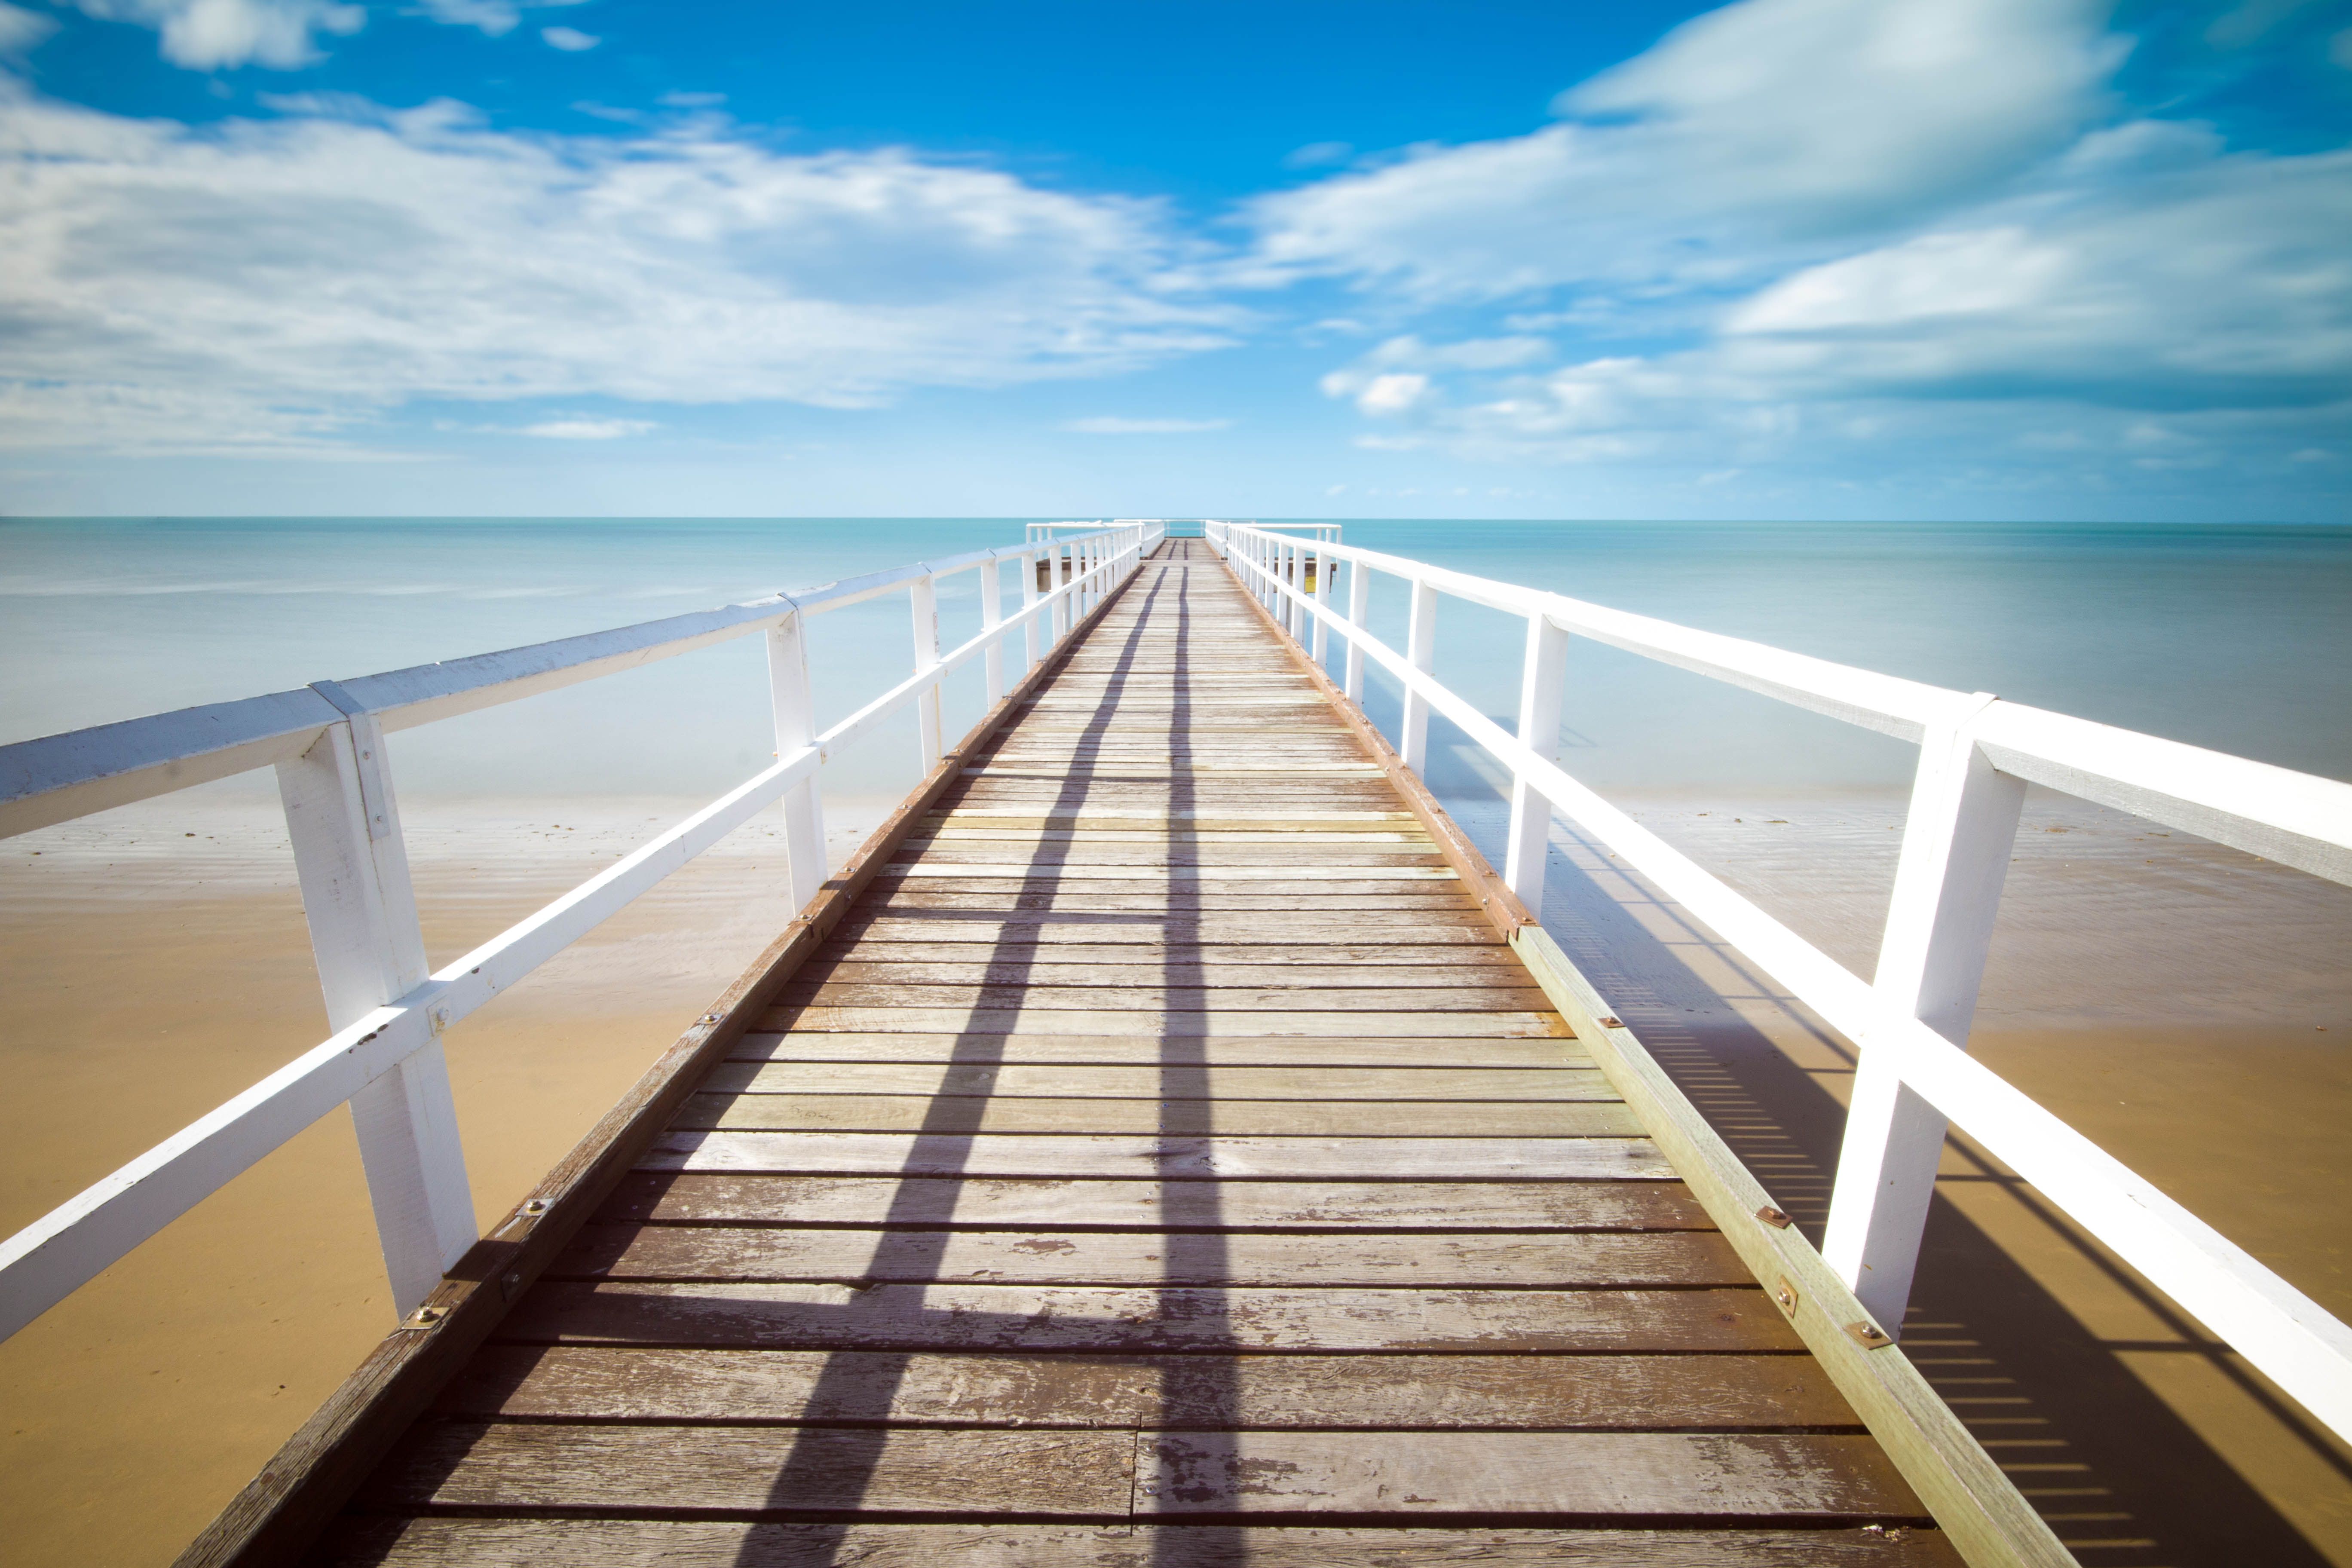
\includegraphics[width=\paperwidth,
                    height=\paperheight]{sf}
}

\subsection{Thanks}


\begin{frame}[c]
%\setsansfont{Birds of Paradise}% the ! did not show
\setsansfont{SoupLeaf}
\ \\ \ \\
\centering \Huge \textcolor{AwesomeYellow}{\textbf{\forbold Thank You!}}
%\centering \Huge \textcolor{green}{\textbf{Thank You!}}
%{Thank You!}
\usebackgroundtemplate{}
\end{frame}

\end{document}
